\documentclass[11pt]{article}
\usepackage[spanish]{babel}
\usepackage[utf8]{inputenc}
\usepackage{listings}
\usepackage{graphicx}
\graphicspath{{Imagenes/}}

\usepackage[paper=portrait, pagesize]{typearea}
\usepackage{titlepic}



\begin{document}

\begin{titlepage}
\centering
\vspace{4.5cm}
{\scshape\LARGE Selección del Sistema Software a Desarrollar y Organización del Grupo de Trabajo \par}
\vspace{1.5cm}


\includegraphics[width=16cm] {../Imagenes/Logo}

\vspace{3cm}
{\scshape\large 29 de Septiembre de 2019\par}
\vspace{1cm}

{Miguel Albertí Pons\\
Sofía Almeida Bruno\\
Pedro Manuel Flores Crespo\\
María Victoria Granados Pozo\\
Lidia Martín Chica
\par}

\end{titlepage}





\newpage
\section {Make A Travel (App)}
Actualmente, viajar está en auge y los paquetes de las compañías están anticuados y poco personalizados. Además, si no quieres acudir a una agencia de viajes, ya que podría incrementar el precio, o dedicar muchas horas a organizar un viaje que se adapte a ti, con esta app pretendemos que a través de las experiencia vividas por otros usuarios puedas planear tu viaje ideal sin salir de la aplicación.

En esta aplicación los usuarios tienen un papel principal, en primer lugar serán ellos los que \textbf{ofertan} sus experiencias y sus actividades, mediante fotos y descripciones, que otros usuarios podrán \textbf{valorar, comentar, seleccionar y personalizar} el viaje.

Las publicaciones de los usuarios podrán ser de distintos tipos como \textbf{rutas} (gastronómicas, turísticas, ...), \textbf{eventos} (musicales, obras de teatro, ...) y \textbf{actividades} (deportivas, culturales, ...). Asímismo un usuario puede crear un \textbf{paquete} en el que agrupe varias publicaciones o seleccionar paquetes hechos y adaptarlos a sus intereses.

Los principales objetivos que queremos cubrir son: la \textbf{facilidad} a la hora de organizar un viaje usando filtros que se amolden a lo que buscamos y basándonos en los comentarios y valoraciones de otros usuarios; \textbf{beneficiar económicamente} a aquellos usuarios cuyas publicaciones sean las mejor valoradas; el \textbf{acceso} a todo tipo de usuarios (con discapacidad, de cualquier edad, ...) a usar la aplicación.

Otras funcionalidades que se podrían incorporar son: \textbf{audioguías} para las actividades culturales; recomendaciones para \textbf{hacer la maleta} según las actividades que se vayan a realizar, el destino o el tiempo.

\section {Roles del grupo de trabajo}
Los roles asignados son los siguientes:

\begin{itemize}
\item{Coordinadora}: Lidia
\item{Catalogadora}: María Victoria
\item{Moderador}: Miguel
\item{Presentadora}: Sofía
\item{Gestor de Calidad}: Pedro

\end{itemize}

\newpage
\KOMAoptions{paper=landscape, pagesize}
\section {Mapa Mental}
\begin{figure}[h]
\centering
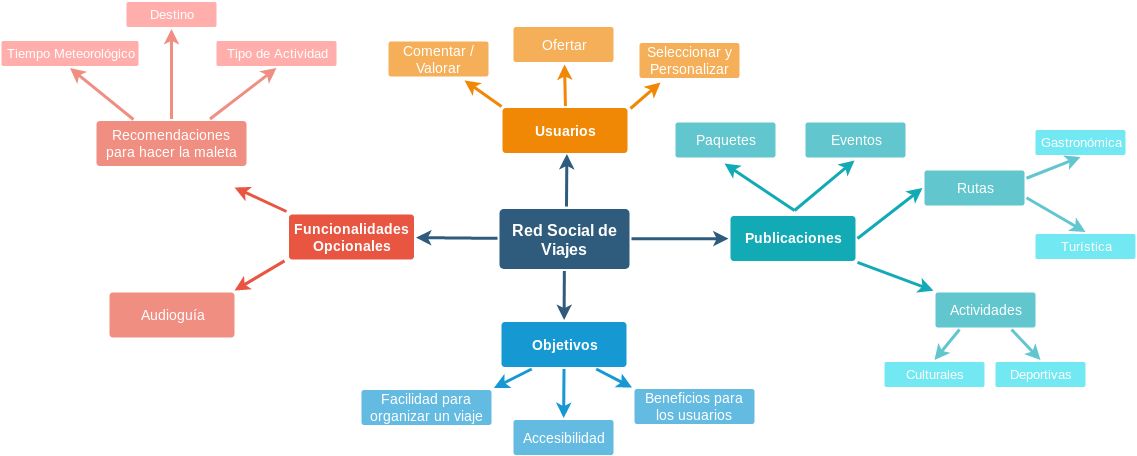
\includegraphics[width=25cm, height=10cm] {../Imagenes/MapaMentalp1}
\end{figure}

\end{document}
